\begin{center}
	\begin{tabular}{|c|c|}
		\hline
		$f_1 = 1 - \frac{\sin{x}}{x}$ & $f_2=x^{10}$ \\
		\hline
		\begin{tikzpicture}[y=3cm, x=.5cm,font=\sffamily]
			%axis
			\draw (0,0) -- coordinate (x axis mid) (10,0);
			\draw (0,0) -- coordinate (y axis mid) (0,0.9);
			%ticks
			\foreach \x in {0,...,10}
			\draw (\x,1pt) -- (\x,-3pt)
			node[anchor=north] {\x};
			\foreach \y in {0,0.3,0.6,0.9}
			\draw (1pt,\y) -- (-3pt,\y) 
			node[anchor=east] {\y}; 
			%labels      
			\node[below=0.8cm] at (x axis mid) {Iteracion};
			\node[rotate=90, above=0.8cm] at (y axis mid) {Error};
			%plots
			\draw plot[mark=*, mark options={fill=white}]
			file {f1_bis.data};
			\draw plot[mark=triangle*, mark options={fill=white} ] 
			file {f1_newt.data};
		\end{tikzpicture}
		&
		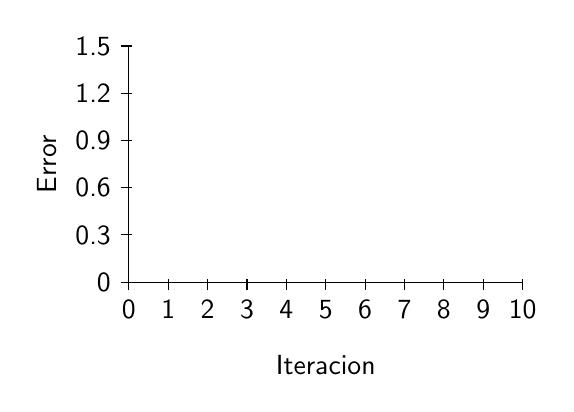
\begin{tikzpicture}[y=2cm, x=.5cm,font=\sffamily]
			%axis
			\draw (0,0) -- coordinate (x axis mid) (10,0);
			\draw (0,0) -- coordinate (y axis mid) (0,1.5);
			%ticks
			\foreach \x in {0,...,10}
			\draw (\x,1pt) -- (\x,-3pt)
			node[anchor=north] {\x};
			\foreach \y in {0,0.3,0.6,0.9,1.2,1.5}
			\draw (1pt,\y) -- (-3pt,\y) 
			node[anchor=east] {\y}; 
			%labels      
			\node[below=0.8cm] at (x axis mid) {Iteracion};
			\node[rotate=90, above=0.8cm] at (y axis mid) {Error};
			%plots
			\draw plot[mark=*, mark options={fill=white}]
			file {f2_bis.data};
			\draw plot[mark=triangle*, mark options={fill=white} ] 
			file {f2_newt.data};
		\end{tikzpicture} \\
		\hline
		\hline
		$f_4 = |x-10|$ & $f_5= - \frac{1}{32} + \frac{5x}{16} - \frac{5x^2}{4}
								+ \frac{5x^3}{2} - \frac{5x^2}{2} + x^5$ \\
		\hline
		\begin{tikzpicture}[y=1.6cm, x=.5cm,font=\sffamily]
			%axis
			\draw (0,0) -- coordinate (x axis mid) (10,0);
			\draw (0,0) -- coordinate (y axis mid) (0,1.5);
			%ticks
			\foreach \x in {0,...,10}
			\draw (\x,1pt) -- (\x,-3pt)
			node[anchor=north] {\x};
			\foreach \y in {0,0.5,1,1.5}
			\draw (1pt,\y) -- (-3pt,\y) 
			node[anchor=east] {\y}; 
			%labels      
			\node[below=0.8cm] at (x axis mid) {Iteracion};
			\node[rotate=90, above=0.8cm] at (y axis mid) {Error};
			%plots
			\draw plot[mark=*, mark options={fill=white}]
			file {f4_bis.data};
			\draw plot[mark=triangle*, mark options={fill=white} ] 
			file {f4_newt.data};
		\end{tikzpicture}
		&
		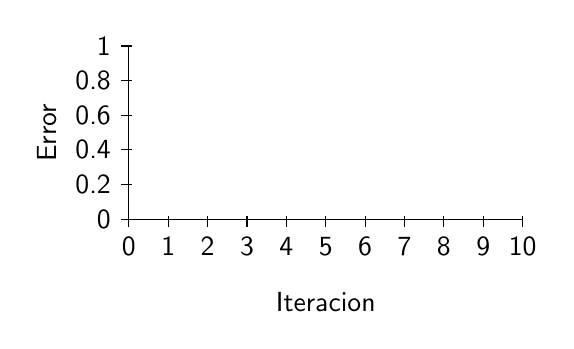
\begin{tikzpicture}[y=2.2cm, x=.5cm,font=\sffamily]
			%axis
			\draw (0,0) -- coordinate (x axis mid) (10,0);
			\draw (0,0) -- coordinate (y axis mid) (0,1);
			%ticks
			\foreach \x in {0,...,10}
			\draw (\x,1pt) -- (\x,-3pt)
			node[anchor=north] {\x};
			\foreach \y in {0,0.2,0.4,0.6,0.8,1}
			\draw (1pt,\y) -- (-3pt,\y) 
			node[anchor=east] {\y}; 
			%labels      
			\node[below=0.8cm] at (x axis mid) {Iteracion};
			\node[rotate=90, above=0.8cm] at (y axis mid) {Error};
			%plots
			\draw plot[mark=*, mark options={fill=white}]
			file {f5_bis.data};
			\draw plot[mark=triangle*, mark options={fill=white} ] 
			file {f5_newt.data};
		\end{tikzpicture} \\
		\hline
		\hline
		$f_6 =$ Bessel primer tipo & $f_7=$ Bassel segundo tipo \\
		\hline
		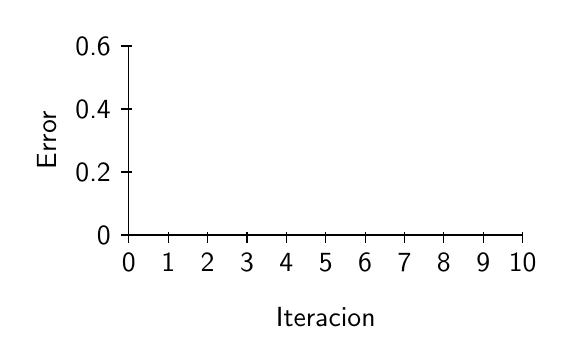
\begin{tikzpicture}[y=4cm, x=.5cm,font=\sffamily]
			%axis
			\draw (0,0) -- coordinate (x axis mid) (10,0);
			\draw (0,0) -- coordinate (y axis mid) (0,0.6);
			%ticks
			\foreach \x in {0,...,10}
			\draw (\x,1pt) -- (\x,-3pt)
			node[anchor=north] {\x};
			\foreach \y in {0,0.2,0.4,0.6}
			\draw (1pt,\y) -- (-3pt,\y) 
			node[anchor=east] {\y}; 
			%labels      
			\node[below=0.8cm] at (x axis mid) {Iteracion};
			\node[rotate=90, above=0.8cm] at (y axis mid) {Error};
			%plots
			\draw plot[mark=*, mark options={fill=white}]
			file {f6_bis.data};
			\draw plot[mark=triangle*, mark options={fill=white} ] 
			file {f6_newt.data};
		\end{tikzpicture}
		&
		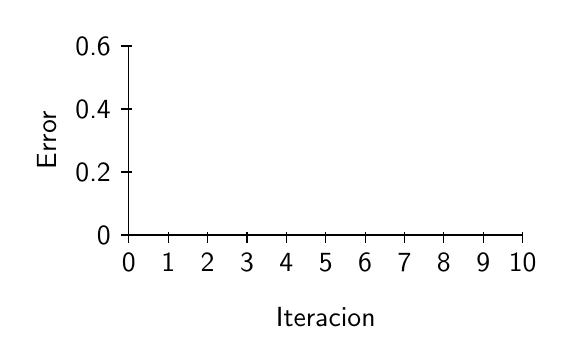
\begin{tikzpicture}[y=4cm, x=.5cm,font=\sffamily]
			%axis
			\draw (0,0) -- coordinate (x axis mid) (10,0);
			\draw (0,0) -- coordinate (y axis mid) (0,0.6);
			%ticks
			\foreach \x in {0,...,10}
			\draw (\x,1pt) -- (\x,-3pt)
			node[anchor=north] {\x};
			\foreach \y in {0,0.2,0.4,0.6}
			\draw (1pt,\y) -- (-3pt,\y) 
			node[anchor=east] {\y}; 
			%labels      
			\node[below=0.8cm] at (x axis mid) {Iteracion};
			\node[rotate=90, above=0.8cm] at (y axis mid) {Error};
			%plots
			\draw plot[mark=*, mark options={fill=white}]
			file {f7_bis.data};
			\draw plot[mark=triangle*, mark options={fill=white} ] 
			file {f7_newt.data};
		\end{tikzpicture} \\
		\hline

	\end{tabular}
\end{center}
